\iffalse %% true for article, false for presentation
\documentclass[12pt]{article}
\usepackage{beamerarticle}
\usepackage[lmargin=1.3in,rmargin=1.3in,tmargin=0.5in,bmargin=0.5in,marginparwidth=1.5in]{geometry}
\else
\documentclass[ignorenonframetext]{beamer}
\fi
\usepackage[export]{adjustbox}
\usepackage{mathptmx}
\usepackage{natbib}
\usepackage{apalike}
\usepackage{multicol}
\usepackage{fancyvrb}
\usepackage{eso-pic}
\usepackage[T1]{fontenc}
\usepackage{tikz}
\usepackage[english]{babel}
\usepackage[latin1]{inputenc}
\usepackage{helvet}
\usepackage{graphicx}
\usepackage{xcolor}
\usepackage{amsmath}
\usepackage{enumitem}

\makeatletter
\gdef\SetFigFont#1#2#3#4#5{%
  \reset@font\fontsize{#1}{#2pt}%
  \fontfamily{#3}\fontseries{#4}\fontshape{#5}%
  \selectfont}%
\makeatother

\setlist[itemize]{itemsep=20pt,label=$\bullet$}

\usepackage{tikz}

\defbeamertemplate<article>{frame begin}{lined}{\par\noindent\rule{\textwidth}{1pt}\par}
\defbeamertemplate<article>{frame end}{lined}{\par\noindent\rule{\textwidth}{1pt}\par}

\newcounter{framebox}
\defbeamertemplate<article>{frame begin}{tikzed}{%
  \par\noindent\stepcounter{framebox}%
  \tikz[remember picture,overlay] %
  \path (-1ex,0) coordinate (frame top \the\value{framebox});}
\defbeamertemplate<article>{frame end}{tikzed}{%
  \hspace*{\fill}\tikz[remember picture,overlay] %
  \draw (frame top \the\value{framebox}) rectangle (1ex,0);\par}


\mode<article>
{
  \setlength{\parskip}{10pt}
  \setlength{\parindent}{0pt}

  \setbeamertemplate{frame begin}[lined]
  \setbeamertemplate{frame end}[lined]
%  \addtobeamertemplate{frame begin}{}{\setbox0=\bgroup}
%  \addtobeamertemplate{frame end}{\egroup}{}
  \usepackage{fancyhdr}
  \renewcommand{\headrulewidth}{0pt}
  \fancypagestyle{plain}{%
    \fancyhead[L]{}
    \fancyhead[C]{}
    \fancyhead[R]{}
    \fancyfoot[C]{}
    \fancyfoot[R]{\raisebox{6in}[0pt][0pt]{\hbox to 0pt{\hspace{0.3in}\framebox{\LARGE\thepage}}}}}
  \pagestyle{plain}
}

\newcommand{\cp}[1]{\textcolor{lightgray}{#1}}
\setcitestyle{authoryear,open={(},close={)}}

\mode<presentation>
{
%  \hypersetup{colorlinks=true,citecolor=green}

  \usecolortheme{default}
  \useinnertheme[shadow]{rounded}
  \useoutertheme{tsinfolines}

  \usesubitemizeitemtemplate{%
    \tiny\raise1.5pt\hbox{\color{beamerstructure}$\blacktriangleright$}%
  }
  \usesubsubitemizeitemtemplate{%
    \tiny\raise1.5pt\hbox{\color{beamerstructure}$\bigstar$}%
  }

  \setbeamersize{text margin left=1em,text margin right=1em}

% Turns off headline.
%  \setbeamertemplate{headline}[default]

  %% started as:  \usetheme[secheader]{Boadilla}
%  \usecolortheme{albatross}
  % or ...

  \setbeamercovered{invisible}
  % or whatever (possibly just delete it)

%  \addtobeamertemplate{frame title}{\begin{center}}{\end{center}}
%  Doesn't seem to do what I'd want.

}

%\beamertemplatenavigationsymbolsempty


\title{VR Graphics Programming for, well, you know}
\subtitle{Some (relatively) easy steps to virtual reality, Part 3}
\author{Tom Sgouros}
\institute{Center for Computation
    and Visualization\\Brown University\\thomas\_sgouros@brown.edu}
\date{Spring 2018}


% If you wish to uncover everything in a step-wise fashion, uncomment
% the following command:

%\beamerdefaultoverlayspecification{<+->}

\begin{document}

\maketitle

\begin{frame}
\titlepage
\end{frame}



\section{Virtual reality}

\begin{frame}{What is virtual reality?}

\begin{center}
\begin{minipage}{0.4\columnwidth}
\begin{center}
Linking the world you made up to the world you live in.
\end{center}
\end{minipage}
\end{center}
\vfill
\begin{minipage}{0.9\columnwidth}
\begin{multicols}{2}

\begin{itemize}

\item Linking head movements to the view matrix.

\item Stereo imagery.

\item Natural interaction modes: pointing, gestures.

\item Immersion.

\end{itemize}
\end{multicols}
\end{minipage}


\end{frame}


\begin{frame}{Input}

\begin{center}
\begin{minipage}{0.8\columnwidth}

\begin{itemize}

\item Asynchronous input plus

\item Continuously tracking equals

\item LOTS of events.
\end{itemize}
\end{minipage}
\end{center}
\end{frame}

\begin{frame}{MinVR}

\begin{center}
\begin{minipage}{0.8\columnwidth}

\begin{description}\raggedright
\setlength{\itemsep}{10pt plus 7pt}
\item[Flexible display structure]  Configurable display node tree.

\item[Flexible events]  You can look at them.

\item[Varying network geometry]  Supports networked, not networked, etc.

\item[Extensible]  Plugin architecture using dynamic libraries.

\item[Configurable] Most network/hardware/graphics changes can be
  accommodated at runtime through a configuration file.

\end{description}


\end{minipage}
\end{center}
\end{frame}




\begin{frame}{MinVR Server/Client Structure}

\begin{center}

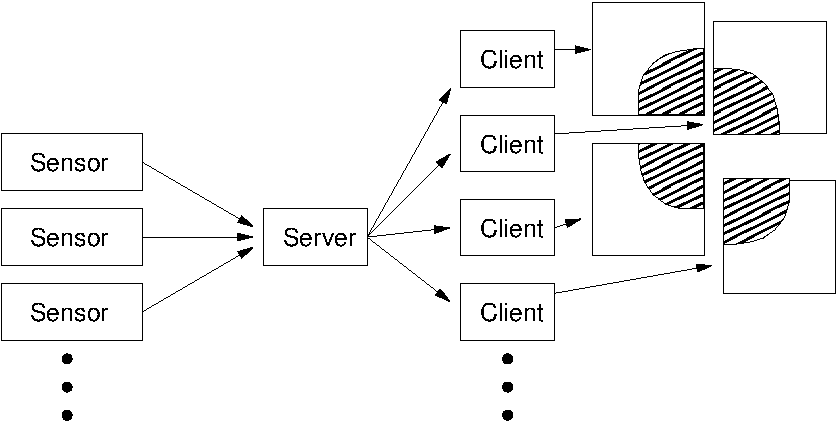
\includegraphics[width=0.9\columnwidth]{images/client-server.pdf}

\end{center}

\hspace{0.2\columnwidth}\begin{minipage}{0.2\columnwidth}
``data''\\
``data''\\
``data''\\
\end{minipage}
\hspace{0.02\columnwidth}\begin{minipage}{0.3\columnwidth}
``Are you ready?''\\
``Here's the data''\\
``Swap''
\end{minipage}

\end{frame}


Data index

\begin{frame}{MinVR Display Graph}

\begin{center}
\begin{minipage}[c]{0.3\columnwidth}
\begin{itemize}\raggedright
\item Simple desktop display on left

\item Stereo YURT nodes on right

\item ``Render'' refers to the user's render function.
\end{itemize}
\end{minipage}\hspace{15pt}
\begin{minipage}{0.51\columnwidth}
\makebox{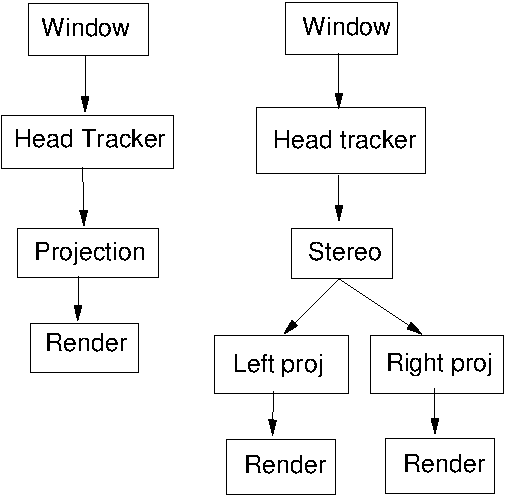
\includegraphics[width=0.99\columnwidth]{images/display-graph.pdf}}
\end{minipage}
\end{center}
\end{frame}




\begin{frame}{MinVR Data Index}

\begin{center}
\begin{minipage}{0.8\columnwidth}

\begin{itemize}\raggedright
\item Hierarchical collection of names and data.

\item Supports VRFloat, VRInt, VRString, VRFloatArray, VRIntArray,
  VRStringArray.

\item And VRContainer, which defines a ``name space.''

\item Use exists() and getValue().

\item Has a ``state'' that can be pushed and popped.

\item Used for events and render state.  Also configuration files,
  using an XML parser.

\end{itemize}

\end{minipage}
\end{center}
\end{frame}



\begin{frame}[fragile]{MinVR Display Graph in practice}

\begin{Verbatim}[fontsize=\scriptsize]
 <displayNode:/MinVR/Desktop/RootNode>
 |   Type: VRGraphicsWindowNode
 |   Values Added:
 |     WindowWidth
 |     WindowHeight
 |   Values Needed:
 |      <none>
 | <displayNode:/MinVR/Desktop/RootNode/HeadTrackingNode>
 |  |   Type: VRHeadTrackingNode
 |  |   Values Added:
 |  |     HeadMatrix
 |  |     CameraMatrix
 |  |   Values Needed:
 |  |      <none>
 |  | <displayNode:/MinVR/D...RootNode/HeadTrackingNode/ProjectionNode>
 |  |  |   Type: VRProjectionNode
 |  |  |   Values Added:
 |  |  |     ViewMatrix
 |  |  |     ProjectionMatrix
 |  |  |   Values Needed:
 |  |  |     CameraMatrix (required)
\end{Verbatim}
\end{frame}






\begin{frame}{MinVR blah blah blah.  How do I use it?}

\begin{center}
\begin{minipage}{0.8\columnwidth}

\begin{itemize}\raggedright
\item Make something to implement the VREventHandler and
  VRRenderHandler interfaces.

\item i.e. write an onVREvent() function, onVRRenderContext(),
  and onVRRenderScene().

\item Create a MinVR::VRMain object, use it to add the event and
  render handlers and initialize it.
\end{itemize}


\end{minipage}
\end{center}
\end{frame}

Display graph

\begin{frame}[fragile]{MinVR Can you be more specific?}

~~~~~~Use MVRDemo.h

\begin{Verbatim}[fontsize=\small]
class MVRDemo : public MinVR::VREventHandler,
  public MinVR::VRRenderHandler {

  typedef MinVR::VRDataIndex VRState;

  MVRDemo(int argc, char** argv);
  virtual void onVREvent(const MinVR::VREvent &eventData);
  virtual void onRenderContext(const VRState& stateData);
  virtual void onRenderScene(const VRState& stateData);

  void run() { while (_main->mainloop()) {} };

  int getLeftoverArgc() { return _main->getLeftoverArgc(); };
  char** getLeftoverArgv() { return _main->getLeftoverArgv(); };
};
\end{Verbatim}
\end{frame}

\begin{frame}[fragile]{MinVR: do it like this}

\begin{Verbatim}[fontsize=\small]
  MVRDemo(int argc, char** argv) {

    _main = new MinVR::VRMain();

    _main->addEventHandler(this);
    _main->addRenderHandler(this);
    _main->initialize(argc, argv);
  }
\end{Verbatim}
\end{frame}

\begin{frame}[fragile]{MinVR event handler}

\begin{Verbatim}
  void onVREvent(const MinVR::VREvent &event) {

    // std::cout << "Hearing event:" << event << std::endl;

    if (event.getName() == "KbdEsc_Down") {
      shutdown();
    } else if (event.getName() == "FrameStart") {
      _oscillator = event.getValue("ElapsedSeconds");
    }
  }
\end{Verbatim}
\end{frame}


\begin{frame}[fragile]{MinVR Events}

~~~~Some typical events:

\begin{Verbatim}[fontsize=\footnotesize]
Hearing event:FrameStart
 | AnalogValue = 10.598754 (float)
 | ElapsedSeconds = 10.598754 (float)
 | EventType = AnalogUpdate (string)

Hearing event:Mouse_Move
 | EventType = CursorMove (string)
 | NormalizedPosition = 0.901563,0.693750 (floatarray)
 | Position = 577.000000,444.000000 (floatarray)

Hearing event:Head_Move
 | EventType = TrackerMove (string)
 | Transform = 0.550934,-0.557136,-0.621348,0.000000,0.727462,0.685475,0.030388,0.000000,0.408... (floatarray)


\end{Verbatim}
\end{frame}

\begin{frame}[fragile]{MinVR render context}

\begin{Verbatim}[fontsize=\small]
  void onVRRenderContext(const VRState &renderState) {

    // std::cout << "entering graphics context:" << renderState << std::endl;

    for (int i = 0; i < _lines.size(); i++) {
      _lines[i].startAnim(plugPos(mrand.get(10),mrand.get(10)));
      _lines[i].step();
    }

    if ((int)renderState.getValue("InitRender") == 1) {
      _checkContext();
      _initializeScene();
      _scene.prepare();
    }
    _scene.load();
  }
\end{Verbatim}
\end{frame}


\begin{frame}[fragile]{MinVR render scene}

\begin{Verbatim}[fontsize=\small]
  void onVRRenderScene(const VRState &renderState) {

      glClear(GL_COLOR_BUFFER_BIT | GL_DEPTH_BUFFER_BIT | GL_STENCIL_BUFFER_BIT);

      std::vector<float> pm =
        renderState.getValue("ProjectionMatrix");
      glm::mat4 proj = glm::mat4( pm[0], pm[1], pm[2], pm[3],
                                  pm[4], pm[5], pm[6], pm[7],
                                  pm[8], pm[9], pm[10],pm[11],
                                  pm[12],pm[13],pm[14],pm[15]);
      ...
      _scene.draw(view, proj);
    }
  \end{Verbatim}
\end{frame}

\begin{frame}[fragile]{Getting and building MinVR}

\begin{Verbatim}[fontsize=\small]
  $ git clone -b beta https://github.com/MinVR/MinVR
  $ cd MinVR
  $ mkdir build
  $ cd build
  $ cmake .. -DWITH_DOCUMENTATION=ON
             -DWITH_PLUGIN_FREEGLUT=ON
             -DWITH_PLUGIN_GLFW=ON
             -DWITH_PLUGIN_OPENGL=ON
  $ make install
\end{Verbatim}

\end{frame}

\begin{frame}[fragile]{Getting and building demo-graphic}


Attach MinVR to your demo-graphic build by defining MINVR\_ROOT to
point to the MinVR \underline{INSTALL} directory.  If you didn't set
it with cmake, this will be in MinVR/build/install.

\begin{Verbatim}[fontsize=\small]
  $ git clone https://github.com/tsgouros/demo-graphic
  $ cd demo-graphic
  $ mkdir build
  $ cd build
  $ cmake .. -DMINVR_INSTALL_DIR=${MINVR_ROOT}
             -DBUILD_DOCUMENTATION=ON
  $ make
\end{Verbatim}

All built?  Try these:

\begin{Verbatim}
  $ bin/treeDemo
  $ bin/objDemoMinVR -c ../config/desktop-freeglut.xml
\end{Verbatim}
\end{frame}




\end{document}
